\begin{frame}
  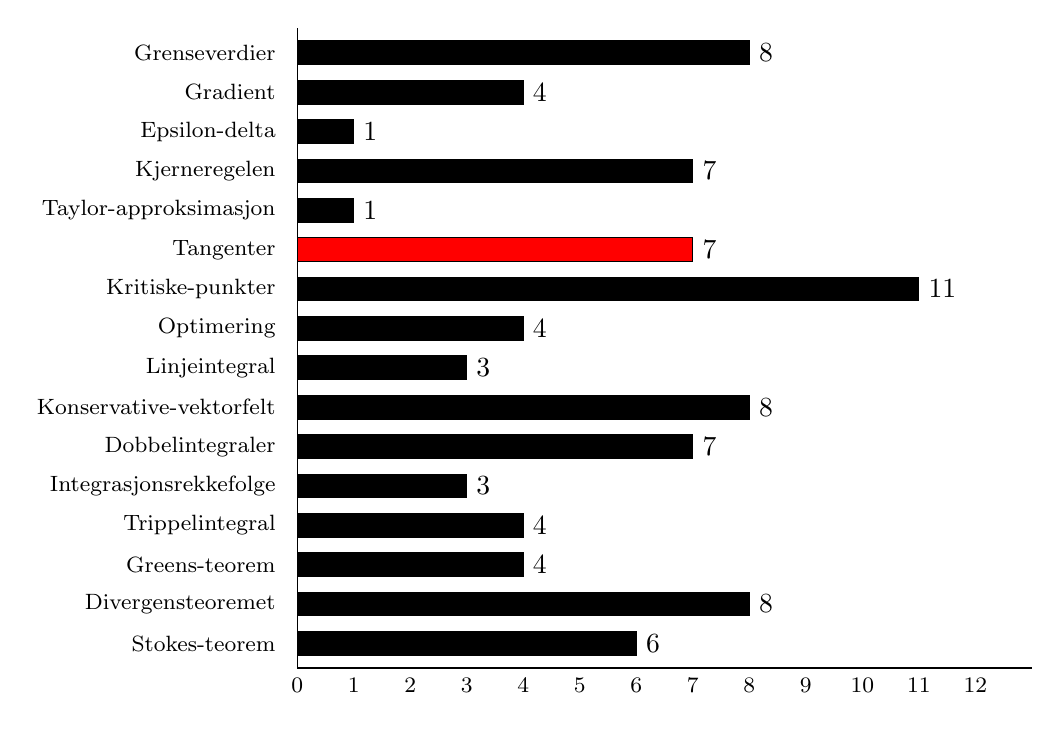
\begin{tikzpicture}
    \begin{axis}[ xbar=0pt, /pgf/bar shift=0pt, legend style={ legend columns=4,
        at={(xticklabel cs:0.5)}, anchor=north, draw=none }, ytick={0,...,15},
      ytick style={draw=none},% <- added
      axis y line*=none, axis x line*=bottom, tick label
      style={font=\footnotesize}, legend style={font=\footnotesize}, label
      style={font=\footnotesize}, xtick style={draw=none},% <- added
      xtick={0,1,...,12}, width=.9\textwidth, bar width=3mm, y dir = reverse,
      xmin=0, xmax=13, area legend,
      y=5mm, enlarge y limits={abs=0.625},
      style={text=black}, every axis plot/.append style={fill},
      nodes near coords, nodes near coords,
      yticklabels={%
        {\topicref{Grenseverdier}},
        {\topicref{Gradient}},
        {\topicref{Epsilon-delta}},
        {\topicref{Kjerneregelen}},
        {\topicref{Taylor-approksimasjon}},
        {\topicref{Tangenter}},
        {\topicref{Kritiske-punkter}},
        {\topicref{Optimering}},
        {\topicref{Linjeintegral}},
        {\topicref{Konservative-vektorfelt}},
        {\topicref{Dobbelintegraler}},
        {\topicref{Integrasjonsrekkefolge}},
        {\topicref{Trippelintegral}},
        {\topicref{Greens-teorem}},
        {\topicref{Divergensteoremet}},
        {\topicref{Stokes-teorem}}}]
      \addplot[fill=black] coordinates {(8,0)};
      \addplot[fill=black] coordinates {(4,1)};
      \addplot[fill=black] coordinates {(1,2)};
      \addplot[fill=black] coordinates {(7,3)};
      \addplot[fill=black] coordinates {(1,4)};
      \addplot[fill=red] coordinates {(7,5)};
      \addplot[fill=black] coordinates {(11,6)};
      \addplot[fill=black] coordinates {(4,7)};
      \addplot[fill=black] coordinates {(3,8)};
      \addplot[fill=black] coordinates {(8,9)};
      \addplot[fill=black] coordinates {(7,10)};
      \addplot[fill=black] coordinates {(3,11)};
      \addplot[fill=black] coordinates {(4,12)};
      \addplot[fill=black] coordinates {(4,13)};
      \addplot[fill=black] coordinates {(8,14)};
      \addplot[fill=black] coordinates {(6,15)};
    \end{axis}
  \end{tikzpicture}
\end{frame}

\begin{frame}
  \subsection{Tangenter}\label{subsec:Tangenter}
  \only<1>{\frametitle{Tangenter}}
  \begin{oppgave}{Matte 2 -- Våren 2010, Oppgave 4b}
    La $f(x,y) = x^3 + y^3 - 3xy$. Skriv opp likningen for tangentplanet til
    grafen til funksjonen $z = f(x,y)$ i punktet $(2,2,4)$. 
  \end{oppgave}
  \textbf{Plan:}
  \begin{enumerate}
    \item Finne normalvektor ved hjelp av gradienten $g(x,y,z) = f(x,y) - z$.
\visible<2->{
      Gradienten er gitt som
      %
      \begin{equation*}
        \nabla g(x,y,z)
        = (\only<2>{\diffp{g}{x}}\only<3>{\diffp{}{x}\left( x^3+y^3-3xy -z\right)}\only<4->{3x^2 - 3y},
          \only<2-4>{\diffp{g}{y}}\only<5>{\diffp{}{y}\left( x^3+y^3-3xy -z\right)}\only<6->{3y^2 - 3x},
          \only<2-6>{\diffp{g}{z}}\only<7>{\diffp{}{z}\left( x^3+y^3-3xy -z\right)}\only<8->{-1})
      \end{equation*}
      %
      \only<8>{Siden gradienten peker i samme retning som normalvektoren setter vi
     $\vek{n} = \nabla g(2,2,4) = (6,6,-1)$.}}
    \item Bruke den generelle likningen for et plan (normalvektor prikket med
      posisjonsvektor) $\vek{n} \cdot (\rr - \rr_0) = 0$.

      \only<9->{Hvor $\vek{\rr} = (x,y,z)$, $\rr_0=(2,2,4)$ og $\vek{n} = (6,6,-1)$
      %
      \begin{align*}
        \only<9>{\vek{n} \cdot (\rr - \rr_0) = 0}
        \only<10>{(6,6,-1) \cdot ( (x-2,y-2,z-4) = 0}
        \only<11>{6(x-2) + 6(y-2) - (z-4)= 0}
        \only<12>{z = 6x + 6y - 20.}
    \end{align*}}
  \end{enumerate}
\end{frame}

%%% Local Variables:
%%% mode: latex
%%% TeX-master: "main"
%%% End:
